\documentclass[12pt]{article}

% Any percent sign marks a comment to the end of the line

% Every latex document starts with a documentclass declaration like this
% The option dvips allows for graphics, 12pt is the font size, and article
%   is the style

\usepackage{amsmath, amssymb}
\usepackage{setspace}
\usepackage{graphicx}
\usepackage{float}
\usepackage[margin=1.0in]{geometry}
\usepackage[font={small,it}]{caption}

% These are additional packages for "pdflatex", graphics, and to include
% hyperlinks inside a document.

%\setlength{\oddsidemargin}{0.25in}
%\setlength{\textwidth}{6.5in}
%\setlength{\topmargin}{0in}
%\setlength{\textheight}{8.5in}
\setlength{\parindent}{0pt}

% These force using more of the margins that is the default style

\begin{document}


\title{Learning Character Graphs from Literature}
\author{Sumit Gogia, Min Zhang, Tommy Zhang}
\date{\today}

\maketitle

\section{Introduction}
    Literary scholars, when comparing different works of literature, frequently use character roles and relationships to make their comparisons. These roles include major single-character literary labels such as ``protagonist'', as well as two-character relationship labels such as ``parent-child''. These character relationships for a novel can be visualized as a graph, an example of which is shown below: 

    \begin{figure}[H]
        \centering
        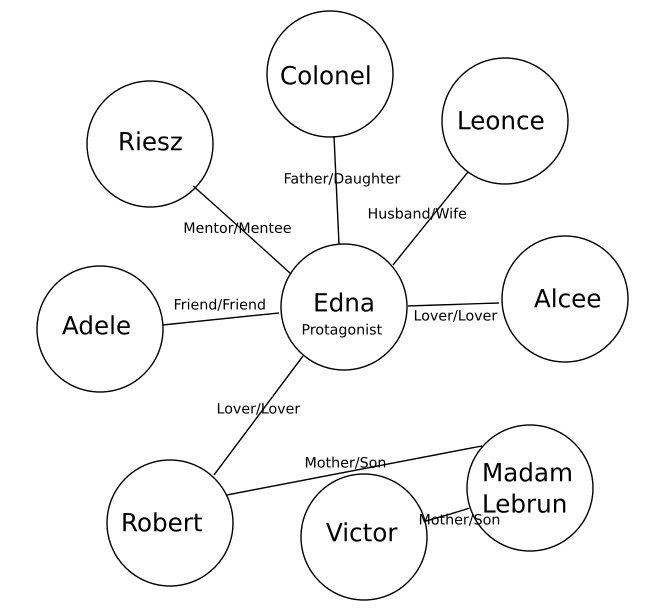
\includegraphics[width=3in]{chara_graph.png}
        \caption{An example character graph for \emph{The Awakening}. Note the role label assigned to the protagonist, Edna, and the relationships described by labeled edges.}
    \end{figure}

    We propose, for this project, to build a system that automatically produces these graphs, which we call \emph{character graphs}, given the text for a work of literature. While literary scholars frequently hypothesize trends in literature by performing a small scale analysis of different works manageable through close reading and manual annotation, having a system that can automatically visualize these character relationships can help with exploring trends across a large number of novels.

\section{Methods}
\subsection{Data Collection}
\subsection{Baseline}
\subsection{Our Approach}
    Our proposed system takes the form of a pipeline of subsystems that extract character references from the text, determine semantic representations of them, and then classify their literary roles and relationships from this semantic representation. The pipeline is visualized below: 
    
    \begin{figure}[H]
        \centering
        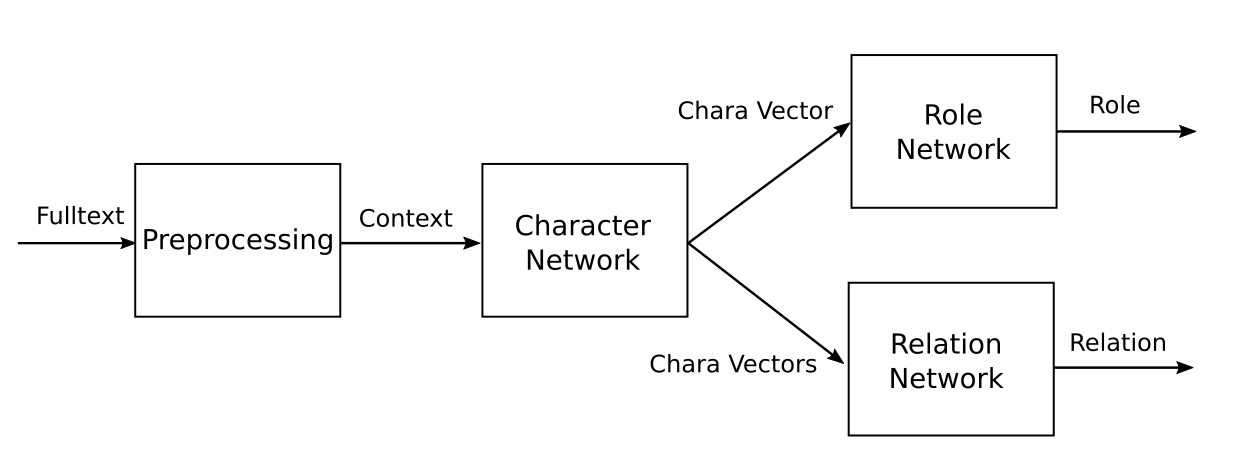
\includegraphics[width=6in]{pipeline.png}
        \caption{The pipeline for the character graph extraction system. \textbf{Note}: the input to preprocessing is the full text, and the output is a list of contexts for \emph{each} possible character. All are used to train the character network.} 
    \end{figure}

    The neural networks we train, for extracting semantic character representations (\emph{character vectors}) and classifying literary relationships, are also visualized separately for clarity: \\ 

    \begin{figure}[H]
        \centering
        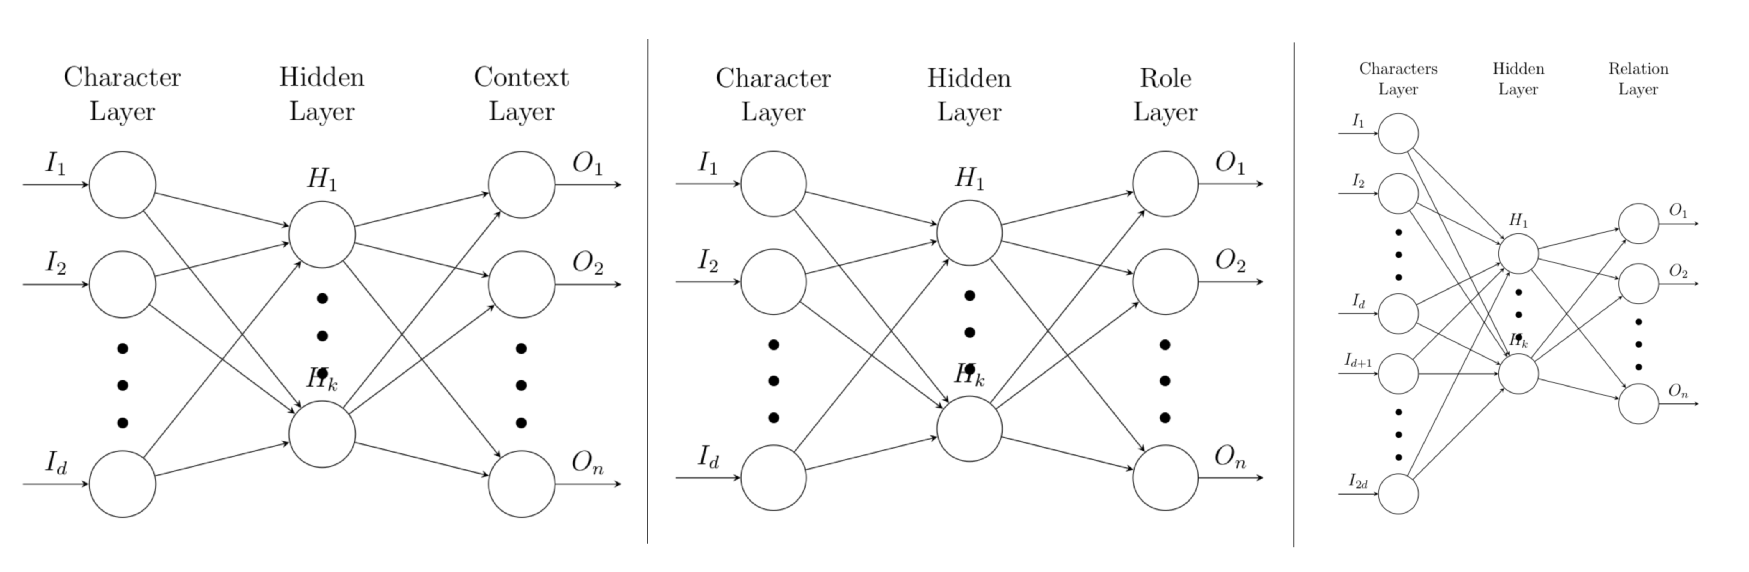
\includegraphics[width=7in]{networks.png}
        \caption{The three neural networks in our pipeline. The left is the character network, which trains character vectors by processing character-context pairs; the middle is the role network, which outputs a role given a character vector; the right is the relation network, which outputs a relation given two character vectors.}
    \end{figure}
    
\subsubsection{Preprocessing}
    Examining the pipeline, we note that the data required for the neural network to train character vectors is a representation of a context for the character. If the character vectors are to be semantically meaningful, it must be that this context, just as when training word vectors, is carefully designed. This is what the preprocessing step is for: to generate a number of context examples for each character. \\

    Exactly what this context should be is unclear; our hope is that taking sentences in which character names appear and extracting action verbs and direct objects will be sufficient for contexts. This might be accomplished by using NER and then matching simple sentences. If this proves insufficient, we can explore other possible contexts, taking into account quotes, or using a dependency parser to extract more detailed features for character-present sentences.

\subsubsection{Networks}
    Each of these networks is trained across the entire dataset of novels obtained from data collection, though we train the character vector network before the other two, as they require semantic character representations as input.  \\

    Our hypothesis is that a semantic character vector can be obtained for each character given context for the character's appearance in a novel, using the first network. Much as word vectors are trained by feeding in word-context pairs, we use this network to train character networks. Given that characters appear many times in these long novels, we believe there is adequate data for learning a representation. \\

    Given output from the first network, the other two networks are similar to many current classification networks using word vectors as input. We feed in a singlet or pair of characters, and then obtain an output label corresponding to their literary role or relationship. To keep learning feasible, we restrict to a small subset of major literary role and prominent relationship labels. Since the training is done over all novels, we believe we will have enough data to perform adequate learning. \\

    After we have passed the characters through the last two networks, we then have labels for each character and a list of labeled 2-character relationships. As described in the introduction, these labels then induce a graph structure that we can visualize. 

\subsection{Result Measuring}
\section{Milestones}

\end{document}
